\subsection{}

Take a look on expression for acceleration, and try to understand, what each term means:

$$\vec{a} = \bigg[\underbrace{\frac{d^2 r}{dt^2}}_{\parbox{2cm}{\scriptsize  \centering v changes \\ due to change of r } } -  \underbrace{r \left(\frac{d\theta}{dt}\right)^2}_{\parbox{2cm}{\scriptsize  \centering centripetal \\ acceleration \\ even if $\omega = const$ }}  \bigg]\hat{r} + \bigg[ 2 \frac{dr}{dt}\frac{d\theta}{dt} +   \underbrace{r\frac{d^2\theta}{dt^2}}_{\parbox{2cm}{\scriptsize  \centering exists even if \\ r = const \\ due to changes \\ in $\omega$}}  \bigg]\hat{\theta}$$

Last term:

$$2 \frac{dr}{dt}\frac{d\theta}{dt} = 2 \cdot \left(\parbox{1.5cm}{\scriptsize  \centering change of \\ radius}\right) \cdot \omega$$

If there is acceleration in direction $\theta$ then there is force in direction $\hat{\theta}$.

If radius increases and there is no forces, then $\omega$ decreases to keep $\frac{dr}{dt}\frac{d\theta}{dt}$ constant:

$$a_\theta = 2 \frac{dr}{dt} + \frac{d\theta}{dt} + r \frac{d^2\theta}{dt^2} = 0 \iff F_\theta = 0$$

$$ \frac{d^2\theta}{dt^2} = \frac{d\omega}{dt} = -\frac{2}{r} \frac{dr}{dt}\frac{d\theta}{dt} = -\frac{2}{r}\frac{dr}{dt}\omega  $$

i.e. change in $\omega$ is of opposite sign to change in $r$.

This is connected to conservation of angular momentum.


\paragraph{Person in falling elevator}

$a_0 = -g$ is system's acceleration

Persons acceleration:

$$\vec{a} = \frac{F_I + F_0}{m} = \frac{F_I}{m} + \frac{F_0}{m}$$

$$\vec{a} = -g + \left[ - \left( a_0 \right)\right] = -g + \left[ - \left( -g \right)\right]  = 0$$

\subsection{Rotating systems}


\begin{center}
	\includegraphics[width=0.5\linewidth]{./lect6/pic1.png}
\end{center}

\paragraph{Connections}

$$\vec{v} \perp \vec{r} \quad \vec{v} \perp \vec{\omega}$$

$$\left| \vec{v} \right| = d \omega = \omega \left| \vec{r}  \right| \sin \left(\frac{\pi}{2} - \theta\right) = \omega \left| \vec{r}  \right| \sin \theta$$


$$\vec{v} = \vec{\omega} \times \vec{r}$$

In rotating system there is imaginary force (centrifugal) out of center:

$$\vec{a} = \omega ^ 2 d \hat{d} $$

In inertial system there is real force inside:

$$\vec{a} = - \omega^2 d \hat{d}$$


\paragraph{General expression}

$$\left| \vec{a} \right| = \omega^2 d = \omega^2 r \sin \theta = \omega\left(\left| \vec{\omega} \times 
\vec{r} \right|\right) \stackrel{\parbox{2cm}{\scriptsize  \centering since vectors are \\ perpendicular}}{=} \left| \omega \times \left( \vec{\omega} \times 
\vec{r} \right) \right|$$

\subparagraph{Direction of centrifugal acceleration}

It's imaginary acceleration. Centrifugal acceleration is out of rotation axis and so is perpendicular to $\vec{\omega}$.

In this example it's also perpendicular to $\vec{v}$. So 

$$\underbrace{\vec{a}_{cen}}_{imaginary} = -\vec{\omega} \times \vec{v} = - \vec{\omega} \times \left( \vec{\omega} \times \vec{r} \right)$$

$\vec{a}$ should be in direction of $\hat{r}$, i.e. $r = const$ and $\omega = const$

\paragraph{}
\begin{center}
	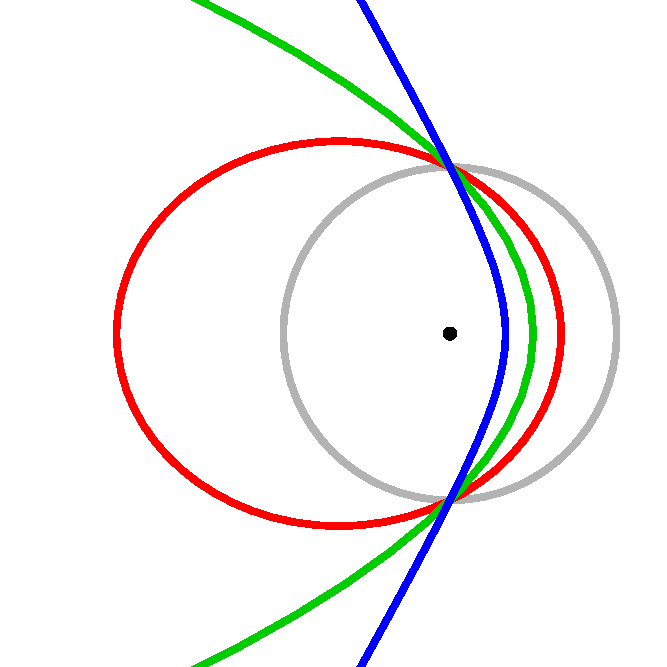
\includegraphics[width=0.5\linewidth]{./lect6/pic2.png}
\end{center}

\begin{enumerate}
	\item Rotating system with angular velocity $\omega$
	\item Mass $m$ with perpendicular velocity (in the system) $v_R$.
	$$\vec{v}_R = v_R \hat{\theta}$$
\end{enumerate}

\subparagraph{Acceleration in inertial system}

$$v_I = \underbrace{\omega r}_{\parbox{2cm}{\scriptsize  \centering  velocity of\\ a point in\\rotating system}} +  \underbrace{v_R}_{\parbox{2cm}{\scriptsize  \centering  velocity of \\ mass relative \\ to a point}}$$

$$\vec{a}_I = -\omega^2_I r \hat{r} \stackrel{\omega_I = \frac{v_I}{r}}{=} -\left(\frac{v_I}{r}\right)^2r\hat{r} = -\hat{r} \frac{\left( \omega r + v_r \right)^2}{r} = \hat{r} \left[ \omega^2 r + \frac{v_R^2}{r} + 2\omega v_R \right]$$

A Person in a rotating system sees a mass moving with a velocity $v_R$. Since relative to him a mass has a tangent speed, he "sees" centripetal acceleration in his frame of reference:

$$\vec{a}_R = -\hat{r} \frac{v^2_R}{r}$$

$$\vec{a}_I = -\hat{r} \frac{v_R^2}{r} - \hat{r}\omega^2r-\hat{r}2\omega v_r $$


$$\vec{a}_R = -\hat{r} \frac{v^2_R}{r} = \vec{a}_I + \underbrace{\hat{r} \omega^2 r}_{\parbox{1.5cm}{\scriptsize  \centering  centrifugal \\ acceleration}} + \underbrace{\hat{r} 2 \omega v_R}_{\parbox{1.5cm}{\scriptsize  \centering  Coriolis \\ acceleration}}$$
